% 第 32 题（源Ⅱ-3）折线段 ABCDE：源为嵌入位图（374×284 @152.3 ppi），
% 按题面坐标等比绘制（1 单位 = 17.87 pt），顶点与标签按源实测（Y = 310 − y_page）。
% 照源要点：两轴仅正方向端有箭头；两轴均越过原点一段（x 轴左伸 3.25 单位、y 轴下伸 2.72 单位，无箭头）；
% 无刻度、无数字；原点与五个顶点各一枚实心点（源内为红点，本项目黑白输出以实心黑点复刻）。
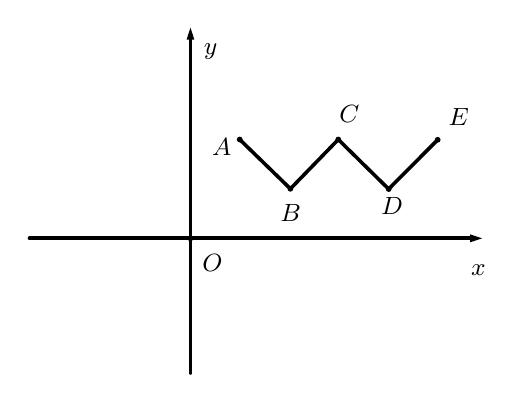
\begin{tikzpicture}[line cap=round,line join=round,font=\small,x=0.03515cm,y=0.03515cm]
% ===== 坐标轴（源线宽约 1.4pt；正方向端实心三角箭头；负方向端无箭头）=====
\draw[line width=1.4pt] (340.3,18.2)--(500.0,18.2);   % x 轴（线体止于箭头基）
\draw[line width=1.4pt] (398.4,-30.4)--(398.4,90.5);  % y 轴
\fill (503.8,18.2)--(499.4,16.75)--(499.4,19.65)--cycle;   % x 轴右端实心箭头
\fill (398.4,94.3)--(397.0,90.0)--(399.8,90.0)--cycle;     % y 轴上端实心箭头
% ===== 折线段（源线宽约 1.3pt）=====
\draw[line width=1.3pt] (416.2,53.9)--(434.5,36.1)--(451.8,53.9)--(470.0,36.0)--(487.7,53.8);
% ===== 实心点（原点与五顶点）=====
\fill (398.4,18.2) circle[radius=1.05pt];
\fill (416.2,53.9) circle[radius=1.05pt];
\fill (434.5,36.1) circle[radius=1.05pt];
\fill (451.8,53.9) circle[radius=1.05pt];
\fill (470.0,36.0) circle[radius=1.05pt];
\fill (487.7,53.8) circle[radius=1.05pt];
% ===== 标签（照源墨迹中心）=====
\node[anchor=center,inner sep=0] at (409.7,51.1) {\(A\)};
\node[anchor=center,inner sep=0] at (434.6,27.2) {\(B\)};
\node[anchor=center,inner sep=0] at (455.8,63.1) {\(C\)};
\node[anchor=center,inner sep=0] at (471.2,30.0) {\(D\)};
\node[anchor=center,inner sep=0] at (495.3,62.2) {\(E\)};
\node[anchor=center,inner sep=0] at (406.4,9.2) {\(O\)};
\node[anchor=center,inner sep=0] at (502.4,6.6) {\(x\)};
\node[anchor=center,inner sep=0] at (405.7,85.8) {\(y\)};
\end{tikzpicture}
